\chapter{Оценка скорости набегающего потока в установившемся режиме движения ПА по изменению параметров работы маршевых движителей}\label{ch:Velocity}

\section{Анализ модели маршевого движителя в установившемся режиме работы}
Как было показано в формулах \ref{eq:kt_kq} в установившемся режиме упор создаваемый гребным винтом движителя $T$ и момент сопротивления вращению $Q$ формируемый при этом на валу определяется следующими формулами:
\begin{gather*}
    T(n, J_0) = K_T (J_0) \rho D^4 n |n|\\
    Q(n, J_0) = K_Q (J_0) \rho D^5 n |n|
\end{gather*}
\noindent где
\begin{itemize}
    \item $K_T (J_0), K_Q (J_0)$ -- соответственно, коэффициенты упора и момента;
    \item $D$ -- диаметр винта;
    \item $\rho$ -- плотность воды;
    \item $n$ -- скорость вращения гребного винта;
\end{itemize}

Переменная $J_0$ представляет собой относительную поступь и определяется следующим уравнением:
\begin{equation*}
    \label{eq:ratio_1}
    J_0 = \frac{v_a}{nD}
\end{equation*}
\noindent где $v_a$ -- скорость набегающего потока воды относительно ПА.
Эта скорость не совсем равна скорости аппарата $v$ и в устоявшемся режиме связана с ней следующим соотношением \cite{lewis1988principles}:
\begin{equation*}
    v_a = (1-w)v
\end{equation*}
\noindent где $w$ -- коэффициент попутного потока.

Более подробно параметр $w$ представлен в работе \cite{10.1016/s1474-6670-17-46514-1} которая опирается лекционные заметки \cite{walderhaug1992motstand}:

\begin{equation*}
    v_a = (1-w)u = (1 - w_w - w_p - w_v)v
\end{equation*}
\noindent где
\begin{itemize}
    \item $w_p$ -- составная часть коэффициента попутного потока отражающая влияние так называемых потенциальных эффектов связанных с влиянием движения корпуса судна или ПА на скорость движения воды;
    \item $w_v$ -- составная часть коэффициента попутного потока отражающая влияние вязких эффектов из-за влияния пограничных слоев.
\end{itemize}

Параметр $w$ находится в диапазоне $0.1-0.4$ в зависимости от конструктивных особенностей судна.
Этот коэффициент важен для движителей судов так как движители там установлены в гидродинамической тени, которую создает корпус судна и учет этого параметра необходим.
При разработке АНПА, за счет малого и обтекаемого корпуса и, зачастую, за счет выноса маршевой группы из гидродинамической тени создаваемой аппаратом, этим коэффициентом можно пренебречь и в дальнейшем в работе мы будем считать что $v_a \approx v$.

Коэффициенты упора и момента гребного винта $K_T (J_0), K_Q (J_0)$ в ограниченных пределах могут быть линейно аппроксимированы следующим образом \cite{10.1109/48.838987}:
\begin{gather}
    \label{eq:coef_1}
    K_T(J_0) = \alpha_1 - \alpha_2 J_0 \\
    K_Q(J_0) = \beta_1 - \beta_2 J_0 
\end{gather}
\noindent где $\alpha_i, \beta_i$ -- безразмерные положительные константы.

Такая линейная аппроксимация позволяет утверждать что коэффициенты $\alpha_1, \beta_1$ определяют эффективность гребного винта при отсутствии набегающего потока.

Таким образом уравнения \ref{eq:coef_1} могут быть переписаны в следующей форме:
\begin{gather}
    K_T = K_T^{bp} - \alpha_1 J_0 \notag \\
    K_Q = K_Q^{bp} - \beta_1 J_0 \label{eq:torque_linear}
\end{gather}
\noindent где $K_T^{bp}, K_Q^{bp}$ -- коэффициенты упора и момента гребного винта полученные в результате швартовых испытаний движителя.

Из определения линейной аппроксимации коэффициента момента (\ref{eq:torque_linear}) и относительной поступи (уравнение \ref{eq:ratio_1}) можно выразить скорость набегающего потока следующим образом:
\begin{equation*}
    v = \frac{1}{\beta_1} n D \left( K_Q^{bp} - K_Q \right)
\end{equation*}

С другой стороны, согласно модели электропривода подводного движителя представленного в выражении \ref{eq:motor_model} в установившемся режиме работы момент сопротивления вращению на валу движителя прямо пропорционален току на его обмотках:
\begin{equation*}
    Q = K_mI
\end{equation*}

% Важно учесть что, при релейном управлении фазами бесколлекторного двигателя коэффициент $K_m$ не является постоянной величиной и имеет обратно экспоненциальную зависимость от времени между переключениями фаз. 
% Эта зависимость хорошо описывается следующим уравнением в установившемся режиме работы мотора:
% \begin{equation}
%     \label{eq:couple_coeff}
%     Q(n, I) = K_m(n)I = F_m \frac{I}{n}
% \end{equation}
% \noindent где $I$ -- ток на обмотках мотора, $n$ -- скорость вращения вала мотора, а переменную $F_m$ будем называть коэффициентом магнитной связности ротора и статора и её считаем величиной постоянной для данной конструкции привода.

% Соответственно, в установившемся режиме работы привода момент на валу мотора пропорционален току на обмотке привода, тогда может быть получено следующее выражение для расчета скорости набегающего потока на гребной винт движителя:

Тогда формула для расчета скорости по параметрам работы движителя будет записана следующим образом:
\begin{equation}
    \label{eq:velocity_final}
    u = \frac{1}{\beta_1} \left( K_Q^{bp} n D - K_m\frac{I}{\rho D^4|n|n} \right)
\end{equation}

\section{Учёт пространственной ориентации маршевых движителей при оценке скорости набегающего потока}
В случае, если подводный аппарат оснащён единственным маршевым движителем, а маневрирование обеспечивается рулями управления в режиме крейсерской скорости или при помощи подруливающих движителей в позиционном режиме или в режиме малых скоростей, то формула \ref{eq:velocity_final} может обеспечить оценку скорости набегающего потока.
Примером таких аппаратов может служить линейка АНПА ``Remus'' \cite{allen1997remus, kukulya2010under}.

С другой стороны, отечественная практика разработки автономных подводных аппаратов отходит от мировой и в основном заключается в использовании четырех движителей, расположенных в кормовой секции под некоторым углом к продольной оси аппарата.
Это такие аппараты как «МТ-2010» \cite{борейко2011малогабаритный}, «ММТ-3000» \cite{горнак2007ммт} и прочие АНПА разработанные в Институте проблем морских технологий ДВО РАН. 

Такой подход позволяет повысить надежность системы за счет отсутствия основного двигателя, поломка которого полностью выведет из строя подводный аппарат.
Кроме этого такая конфигурация движительно-рулевого комплекса позволяет обеспечивать управление по вращательным степеням свободы даже в позиционном режиме.

В этом расчёт скорости набегающего потока по изменению параметров работы электроприводов более затруднителен и требует точного учета расположения и ориентации каждого движителя в пространстве.

Пусть движители повёрнуты относительно продольной оси аппарата на углы $\phi^i, \theta^i$, где угол $\phi^i$ определяет разворот движителя в горизонтальной плоскости, а $\theta^i$ -- разворот движителя в вертикальной плоскости.
Идентификатор $i$ меняется в диапазоне $[1,..,k]$, где $k$ -- количество движителей в кормовой секции.

В таком случае расчет скорости набегающего потока на АНПА будет следующим:
\begin{equation}
    \label{eq:velocity_orientation}
    u^i = \frac{u^i_t}{\cos{\psi^i_t}\cos{\theta^i_t}}
\end{equation}
\noindent где
\begin{itemize}
    \item $u^i$ -- скорость набегающего потока на АНПА, т.е. это определяет скорость движения АНПА относительно воды;
    \item $u^i_t$ -- скорость набегающего потока на движитель $i$;
    \item $\psi^i_t$ -- отклонение движителя от продольной оси аппарата в горизонтальной плоскости;
    \item $\theta^i_t$ -- отклонение движителя от продольной оси аппарата в вертикальной плоскости плоскости;
\end{itemize}

% Но такая конфигурация маршевой группы движителей позволяет определять не только скорость набегающего потока, как в случае единственного маршевого движителя, но так же и углы атаки и дрейфа.

% Пусть аппарат оснащен симметричной маршевой группой, состоящей из двух вертикальных и двух горизонтальных движителей.
% Каждый из отклонён от продольной оси аппарата на $\delta$. 
% Пусть на аппарат набегает поток величиной $u$ и при этом угол атаки ПА в ССК $\alpha$ и угол дрейфа $\beta$.
% В этом случае скорости детектиуремые на движителях определяются следующими зависимостями:
% \begin{equation*}
%     \left\{
%     \begin{array}{l}
%         v_l = v \cos{(\delta - \beta)} \\
%         v_r = v \cos{(\delta + \beta)} \\
%         v_u = v \cos{(\delta - \alpha)} \\
%         v_d = v \cos{(\delta + \alpha)}
%     \end{array}
%     \right.
% \end{equation*}

% Из представленной системы уравнений несложно получить что угол атаки и угол дрейфа можно описать следующими выражениями:

% \begin{gather}
%     \alpha = \arctan{\left[\frac{1}{\tan{\delta}}\frac{v_u-v_d}{v_u+v_d}\right]} \\
%     \beta = \arctan{\left[\frac{1}{\tan{\delta}}\frac{v_l-v_r}{v_l+v_r}\right]}
% \end{gather}

% \begin{notequestion}
%     А вот эти уравнения надо проверять.
% \end{notequestion}

% Кроме этого, так же важно учесть, что при наличии ненулевых углов атаки $\alpha$ и дрейфа $\beta$ в скоростной системе координат идентифицируемые скорости на различных движителях будут различны и это необходимо учитывать.

% Пусть АНПА движется со скоростью $u$ относительно грунта с курсом $\phi$ в локальной инерциальной системе координат и постоянным дифферентом вызванным положительной плавучестью АНПА $\theta_b$.

% Пусть течение в области движения АНПА неизменно по скорости и направлению и определяется переменными $u_c$ и $\phi_c$ В ИСК, соответственно.

% \begin{noteplan}
%     Тут еще не доработано. Добавлю про расчет угла атаки и дрейфа и возможность расчета параметров течения, если есть данные с доплера.
% \end{noteplan}

\section{Экспериментальное исследование разработанного метода оценки скорости набегающего потока по данным запусков АНПА ``ММТ-3000''}
В рамках исследования была проверена гипотеза о работоспособности метода оценки скорости набегающего потока по изменению параметров работы приводов маршевых двигателей.

Для этого этого были проанализированы стендовые и маршевые испытания движителей маршевой группы АНПА ``ММТ-3000'', а так же проанализированы данные тестовых запусков подводного аппарата в рамках которых были идентифицированы ГДХ аппарата.

\begin{figure}[ht]
    \centering
    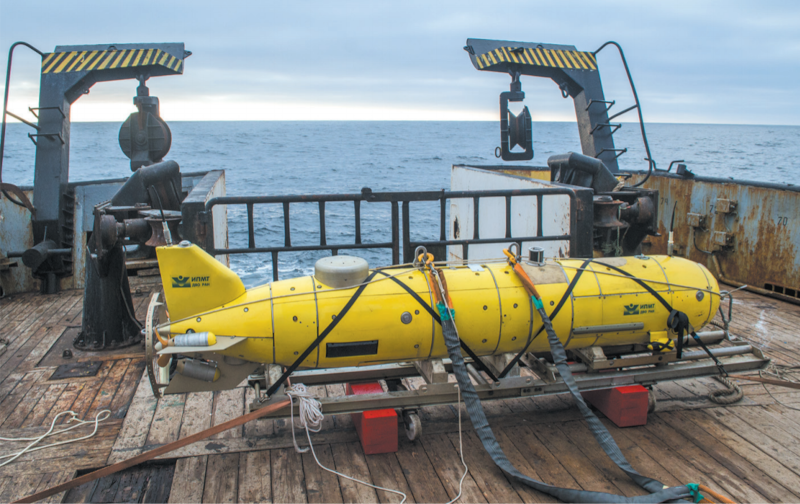
\includegraphics[width=0.8\linewidth]{velocity/MMT3000 - общий вид.png}
    \caption{Общий вид аппарата АНПА ``ММТ-3000''.}
    \label{fig:mmt-3000}
\end{figure}

\begin{table}
    \caption{Параметры углов отклонения движителей маршевой группы АНПА ``ММТ-3000'' от продольной оси аппарата.}
    \label{tab:mmt3000_propulsion_angles}
    \centering
    \begin{tabular}{lll}
        \toprule
        Тип движителя & Угол по горизонтали $\psi$, $^{\circ}$  & Угол по вертикали $\theta$, $^{\circ}$ \\
        \midrule
        Левый  & -11.25 & 3 \\
        Правый &  11.25 & 3 \\
        Нижний &  -22.5 & 0 \\
        \bottomrule
    \end{tabular}
\end{table}

Маршевая секция подводного аппарата состоит из трех движителей.
Два из них расположены симметрично под углом $\psi_l$ и $\psi_r$ к продольной оси аппарата в горизонтальной плоскости и небольшим углом в вертикальной плоскости, $\theta_l$ и $\theta_r$ соответственно.
Последний, нижний, расположен расположен под углом $\theta_v$ к продольной оси аппарата в вертикальной плоскости.
Параметры углов наклона маршевых движителей представлены в таблице \ref{tab:mmt3000_propulsion_angles}.

\subsection{Идентификация параметров работы привода движителя}
В качестве привода маршевого движителя АНПА ``ММТ-3000'' использовался электродвигатель ``2 ДБМ 70-1,1-1,3-3'' производства ОАО «Машиноаппарат».
Параметры электродвигателя приведены в таблице \ref{tab:mmt300_motor}

\begin{table}
    \caption{Параметры электродвигателя ``2 ДБМ 70-1,1-1,3-3'' }\label{tab:mmt300_motor}
    \centering
    \begin{tabular}{ll}
        \toprule
        Наименование параметра  & Значение\\
        \midrule
        Число пар полюсов & 8 \\
        Число фаз & 3 \\
        Номинальное напряжение питания, В   & 24 \\
        Частота вращения при идеальном холостом ходе, об/мин & 1350-1650 \\
        Пусковой момент, Н $\cdot$ м, не менее      & 6,0 \\
        Сопротивление секции фазы (фазы) постоянному току, Ом & 0,165-0,202 \\
        Электромагнитная постоянная времени фазы, мс & 0,4 \\
        Коэффициент момента $K_m$, Н$\cdot$м/А   & 0,065-0,080   \\
        Момент инерции ротора, кг$\cdot$м$^2$   & 2,5$\cdot$10$^{-4}$ \\
        \bottomrule
    \end{tabular}
\end{table}
На рисунке \ref{fig:motor_load_test} продемонстированы результаты проведения нагрузочных испытаний электродвигателя.
Хоть зависимость между моментом на валу электропривода и значением тока на обмотках мотора зависит явно линейно, коэффициент момента $K_m$ различен для разных значений кода управления.
Это поведение хорошо описывается уравнением:
\begin{equation*}
    K_m(k) = \frac{K_m^0}{k}
\end{equation*}
\noindent где $K_m^0$ -- некоторая постоянная, а $k$ -- код управления электроприводом.
Результаты аппроксимации значения коэфициента момента от кода управления для $K_m^0 = 15.2$ приведены на рисунке \ref{fig:function_cm}.

\begin{figure}[ht]
    \centering
    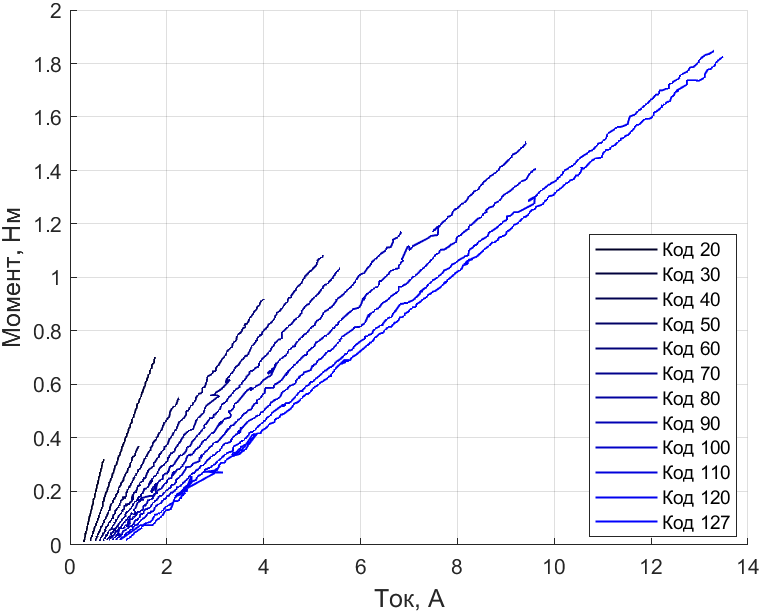
\includegraphics[width=0.8\linewidth]{velocity/MMT3000 - Нагрузочные испытания.png}
    \caption{Результаты нагрузочных испытаний электропривода ``2 ДБМ 70-1,1-1,3-3''.}
    \label{fig:motor_load_test}
\end{figure}

\begin{figure}[ht]
    \centering
    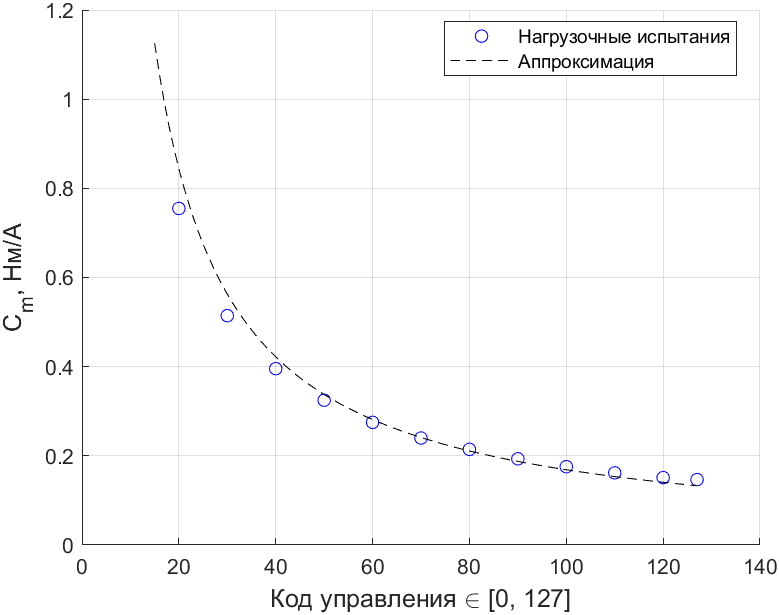
\includegraphics[width=0.8\linewidth]{velocity/MMT3000 - Cm от кода управления.png}
    \caption{Зависимость коэфициента момента электропривода от кода управления $k$.}
    \label{fig:function_cm}
\end{figure}

\subsection{Параметры гребного винта}
В качестве гребного винта на АНПА ``ММТ-3000'' был использован специально изготовленный трехлопастной винт.
Первичные гидродинамические коэффициенты винта $K_T, K_Q$ определены в соответствии с методикой Дайдолла.
Они показаны на рисунке \ref{fig:mmt3000_propeller} вместе с их линейной аппроксимацией в диапазоне относительной поступи 0-0.5, где 0.5 соответствует скорости АНПА примерно 1,5 м/с и скорости вращения гребного винта 22 об/сек.
Все основные параметры гребного винта представлены в таблице \ref{tab:mmt3000_propeller}.

\begin{table}
    \caption{Параметры гребного винта движителей маршевой группы АНПА ``ММТ-3000''
    }
    \label{tab:mmt3000_propeller}
    \centering
    \begin{tabular}{ll}
        \toprule
        Наименование параметра  & Значение\\
        \midrule
        Количество лопастей & 3 \\
        Диаметр, м & 0,19 \\
        Дисковое отношение & 0,40 \\
        Шаговое отношение & 0,87 \\
        Регрессионный $K_T$ & $-0.0964J_0^2 -0.2774J_0 + 0.3519$ \\
        Регрессионный $K_Q$ & $-0.0144J_0^2 -0.0301J_0 + 0.0456$ \\
        Регрессионный $K_T^{lin}$ & $-0.3256J_0 + 0.3558$ \\
        Регрессионный $K_Q^{lin}$ & $-0.0373J_0 + 0.0462$ \\
        \bottomrule
    \end{tabular}
\end{table}

\begin{figure}[ht]
    \centering
    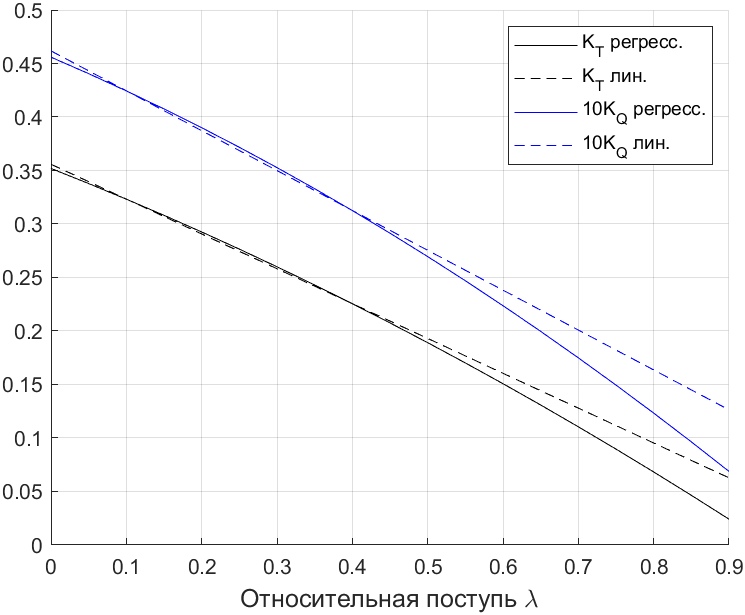
\includegraphics[width=0.8\linewidth]{velocity/MMT3000 - ГВ регресс.png}
    \caption{Параметры ГВ полученные регрессионным анализом.}
    \label{fig:mmt3000_propeller}
\end{figure}

\subsection{Анализ результатов швартовных испытаний маршевых движителя}
В рамках исследования был проведён анализ результатов швартовных испытаний движителя, в результате чего были получены значения усилия создаваемые движителем и потребляемый при этом ток в зависимости от задаваемого кода управления.

Код управления движителем представляет собой целое число находящееся в пределах от -127 до 127, где диапазон от 0 до 127 пропорционально изменяет эффективное значение фазного напряжения на моторе в диапазоне от 0 до 24В, а диапазон от 0 до -127 формирует аналогичное напряжение но с обратным направлением вращения вала мотора.

На рисунке \ref{fig:mmt3000_bollardpul} показана величина упора создаваемого движителем от значения кода управления публикуемого в систему управления движителем.
\begin{figure}[ht]
    \centering
    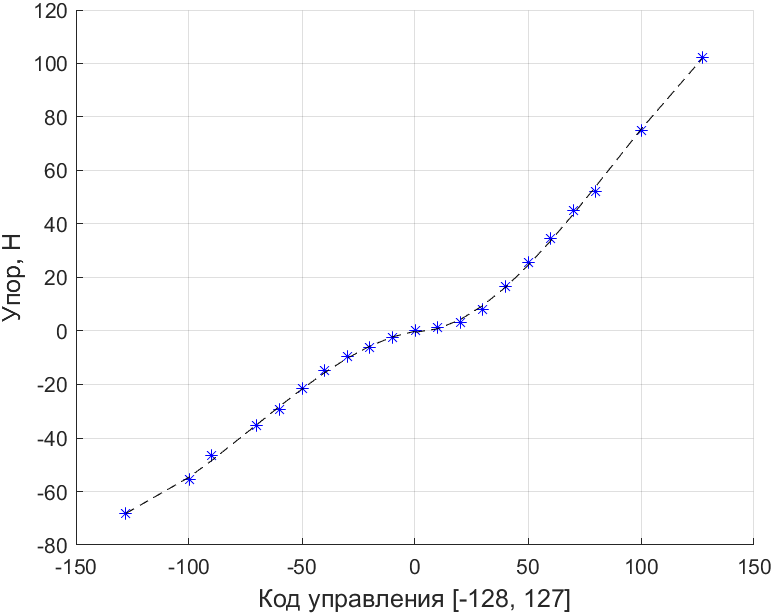
\includegraphics[width=0.8\linewidth]{velocity/MMT3000 - швартовные испытания движителя.png}
    \caption{Статическая характеристики движителя в швартовном режиме.}
    \label{fig:mmt3000_bollardpul}
\end{figure}

Кроме того была рассчитана зависимость создаваемого упора создаваемого гребным винтом (\ref{fig:mmt3000_thrust_rotation2}) и его момента сопротивления вращению (\ref{fig:mmt3000_torque_rotation2}) от квадрата скорости вращения винта для расчёта истинных величин $K_T,K_Q$.

\begin{figure}[ht]
    \centering
    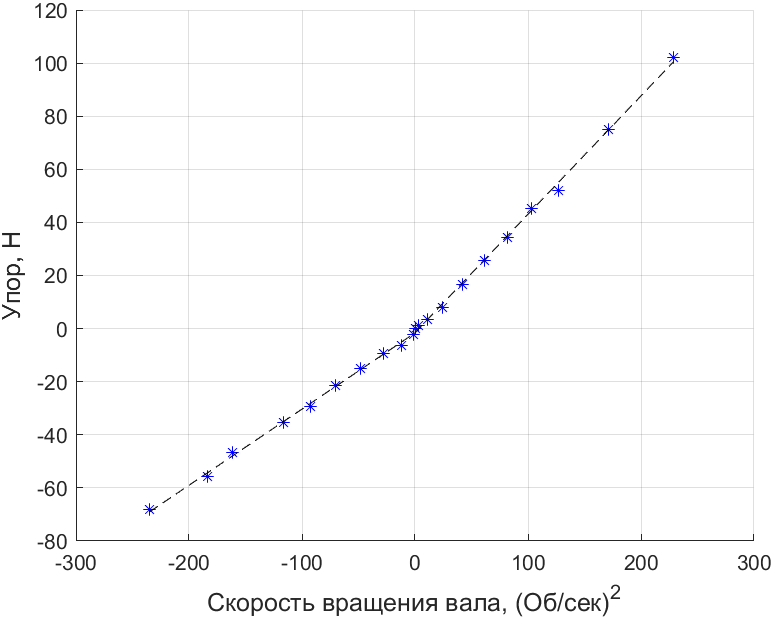
\includegraphics[width=0.8\linewidth]{velocity/MMT3000 - Зависимость упора от 2скорости.png}
    \caption{Зависимость упора создаваемого гребным винтом от квадрата скорости вращения гребного винта.}
    \label{fig:mmt3000_thrust_rotation2}
\end{figure}

\begin{figure}[ht]
    \centering
    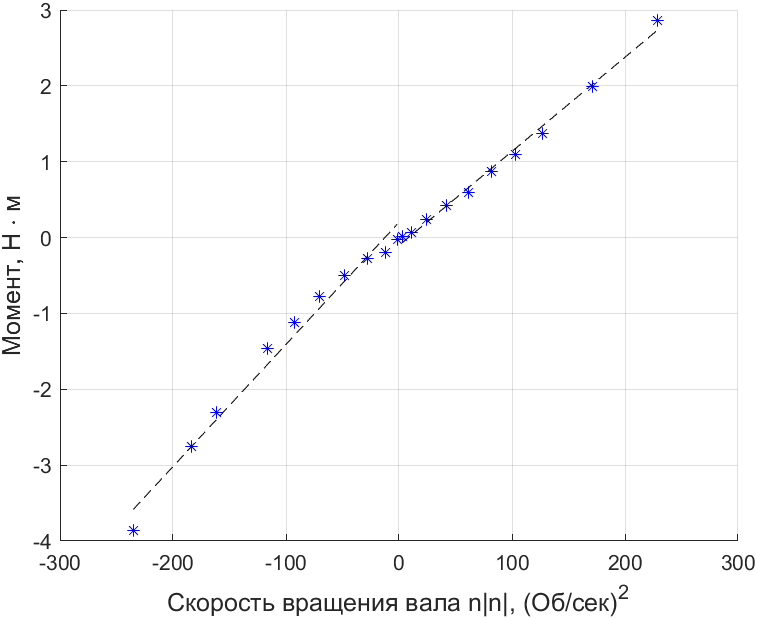
\includegraphics[width=0.8\linewidth]{velocity/MMT3000 - Зависимость момента от 2скорости.png}
    \caption{Зависимость момента сопротивления вращению создаваемого гребным винтом от квадрата скорости вращения гребного винта.}
    \label{fig:mmt3000_torque_rotation2}
\end{figure}

По этим данным были уточнены параметры коэффициентов $K_T, K_Q$ в части $J_0 = 0$, то есть при отсутствии набегающего потока.
На рисунках \ref{fig:mmt3000_propeller_kt_bollard} и \ref{fig:mmt3000_propeller_kq_bollard} соответственно отображены уточненные по результатам швартовных испытаний движителя зависимости коэффициента упора винта $K_T$ и его коэффициента момента сопротивления вращению $K_Q$.
Численные значения уточненных линеаризованных параметров гребного винта представлены в таблице \ref{tab:mmt3000_propeller_bollard}.

\begin{table}
    \caption{Уточненные линеаризованные параметры гребного винта движителей маршевой группы АНПА ``ММТ-3000''.}
    \label{tab:mmt3000_propeller_bollard}
    \centering
    \begin{tabular}{ll}
        \toprule
        Наименование параметра  & Значение\\
        \midrule
        $K_T^{lin}$ & $-0.3256J_0 + 0.3421$ \\
        $K_Q^{lin}$ & $-0.0373J_0 + 0.0501$ \\
        \bottomrule
    \end{tabular}
\end{table}

\begin{figure}[ht]
    \centering
    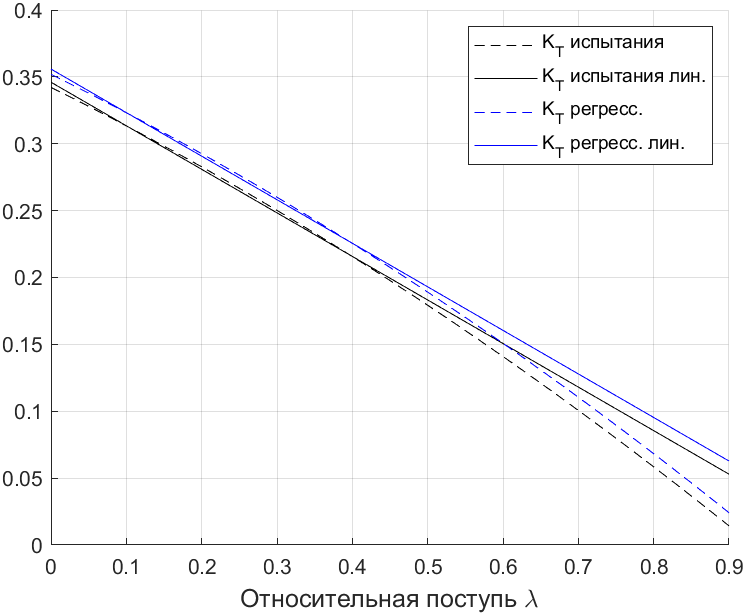
\includegraphics[width=0.8\linewidth]{velocity/MMT3000 - ГВ Kt испытания.png}
    \caption{Коэффициент упора винта $K_t$ с поправкой на результаты швартовных испытаний.}
    \label{fig:mmt3000_propeller_kt_bollard}
\end{figure}

\begin{figure}[ht]
    \centering
    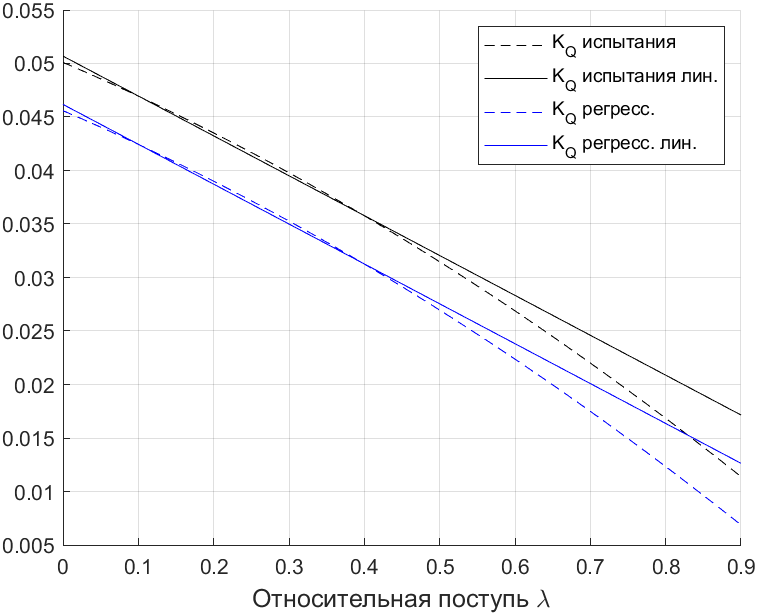
\includegraphics[width=0.8\linewidth]{velocity/MMT3000 - ГВ Kq испытания.png}
    \caption{Коэффициент момента сопротивления вращению винта $K_q$ с поправкой на результаты швартовных испытаний.}
    \label{fig:mmt3000_propeller_kq_bollard}
\end{figure}

\subsection{Анализ гидродинамических характеристик АНПА по результатам натурных испытаний}
В качестве данных для анализов использовались калибровочные запуски АНПА ``ММТ-3000'' для расчета ГДХ подводного аппарата, полученные в 2019 году в заливе Патрокл.
Для расчета ГДХ были проведены запуски подводного аппарата на фиксированной глубине со ступенчатым изменением скорости продольного движения.
График изменения скорости представлен на рисунке \ref{fig:mmt3000_velocity} и соответствующее изменение относительной поступи винта с поправкой на пространственную ориентацию движителей представлена на рисунке \ref{fig:advance_ratio}.

\begin{figure}[ht]
    \centering
    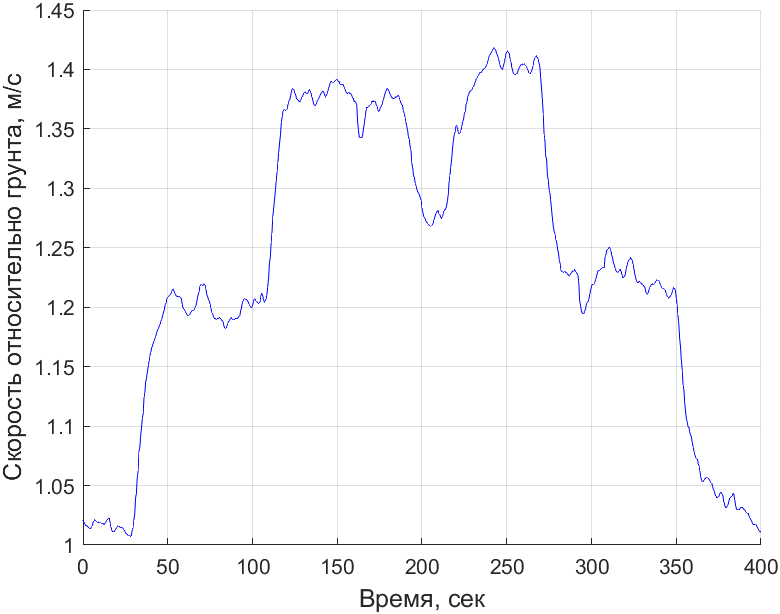
\includegraphics[width=0.8\linewidth]{velocity/MMT3000 - Скорость с допплера.png}
    \caption{Изменение скорости АНПА ``MMT-3000'' на всем маршруте движения.}
    \label{fig:mmt3000_velocity}
\end{figure}

\begin{figure}[ht]
    \centering
    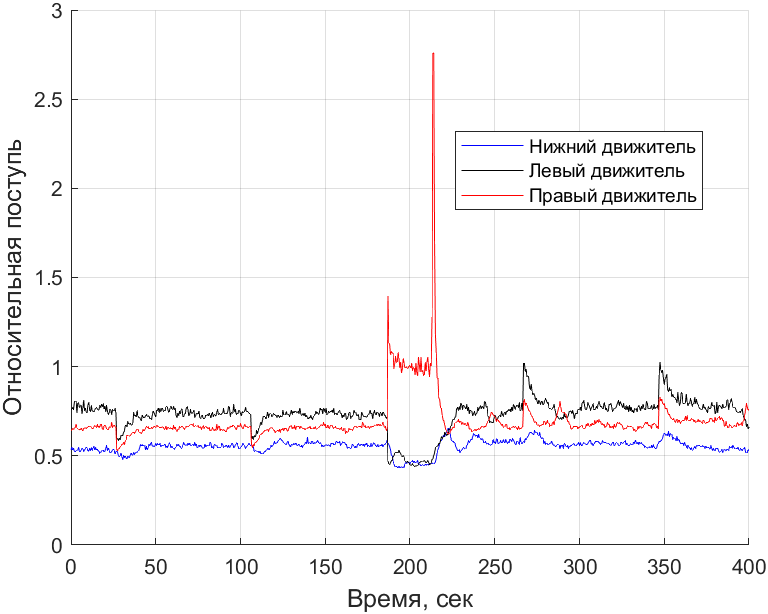
\includegraphics[width=0.8\linewidth]{velocity/MMT3000 - Относительная поступь.png}
    \caption{Значение относительной поступи ГВ маршевой группы движителей АНПА ``MMT-3000'' на всем маршруте движения.}
    \label{fig:advance_ratio}
\end{figure}


Соответствующие ему график изменения потребляемого тока и скорости вращения гребных винтов движителей маршевой группы представлены на рисунках \ref{fig:mmt3000_curent} и  \ref{fig:mmt3000_rotation}, соответсвенно.

\begin{figure}[ht]
    \centering
    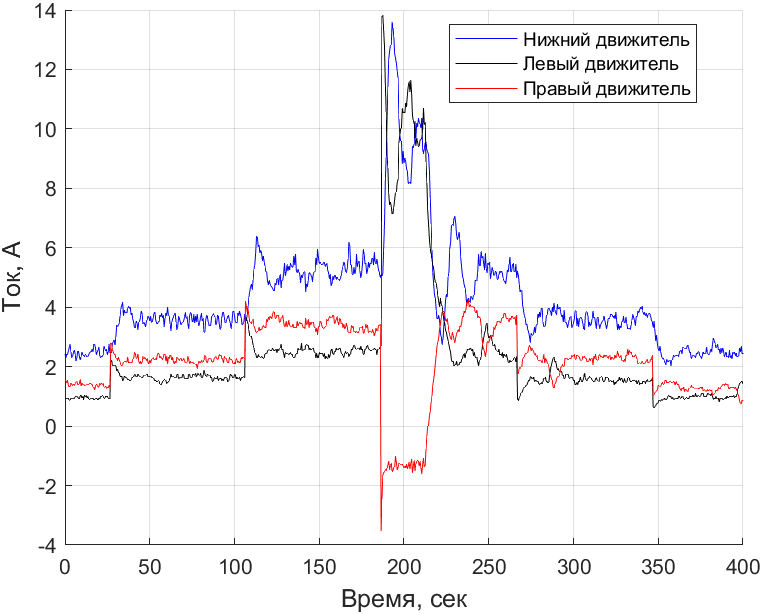
\includegraphics[width=0.8\linewidth]{velocity/MMT3000 - Токи движителей.png}
    \caption{Ток на обмотках электроприводов маршевой группы движителей АНПА ``MMT-3000''.}
    \label{fig:mmt3000_curent}
\end{figure}

\begin{figure}[ht]
    \centering
    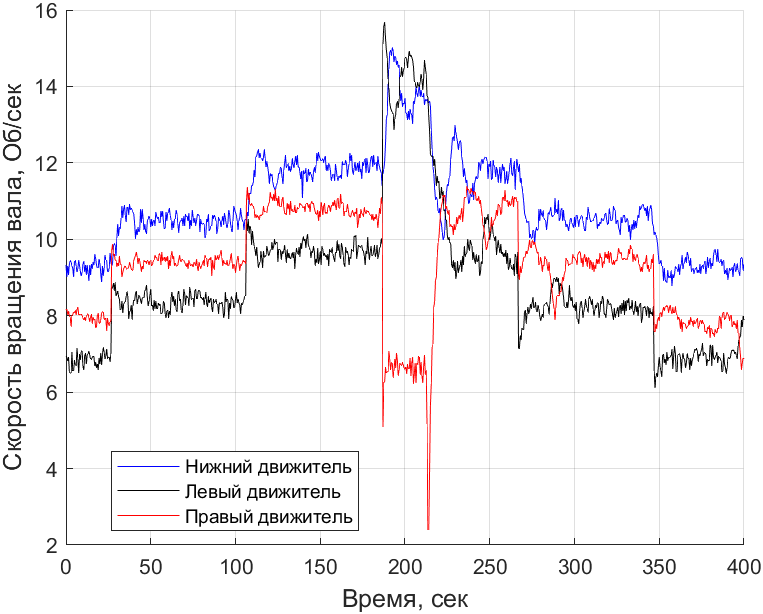
\includegraphics[width=0.8\linewidth]{velocity/MMT3000 - Обороты движителей.png}
    \caption{Скорости вращения гребных винтов движителей маршевой группы подводного аппарата ``MMT-3000''.}
    \label{fig:mmt3000_rotation}
\end{figure}

По первой части движения АНПА (время от 0 до 185 секунд) был откалиброван параметр $\beta_1$, который представляет собой линейный коэффициент полиномиальной аппроксимации коэффициента сопротивления вращению гребного винта $K_Q$. 

Была использована выведенная формула расчета скорости набегающего потока \ref{eq:velocity_final} с учётом геометрии движительно-рулевого комплекса (уравнение \ref{eq:velocity_orientation}).
Для этого по методу наименьших квадратов был рассчитан такой параметр $\beta_1$ при котором минимизируется следующая разница:
\begin{equation}
    \label{eq:b1_search}
    min\left\{ \sum_{i=0}^N\left( v_d - v_i \right)^2 \right\}
\end{equation}
\noindent где
\begin{itemize}
    \item $N$ -- количество движителей маршевой группы;
    \item $v_d$ -- продольная скорость движения АНПА полученная от датчика доплеровского лага;
    \item $v_i$ -- скорость полученная согласно выражению \ref{eq:velocity_final} по параметрам работы движителей $i$-го движителя маршевой группы.
\end{itemize}

По данному методу коэффициент $\beta_1$ составил 0.0301 (по расчетам в рамках регрессионного анализа для данной геометрической конфигурации гребного винта данный коэффициент составил 0.0363).

На рисунке \ref{fig:mmt3000_velocity_test} показан график скорости продольного движения АНПА ``ММТ-3000'' полученный разными методами на тестовом участке движения от 0 до 185 секунд после уточнения параметра $\beta_1$ по формуле \ref{eq:b1_search}.

\begin{figure}[ht]
    \centering
    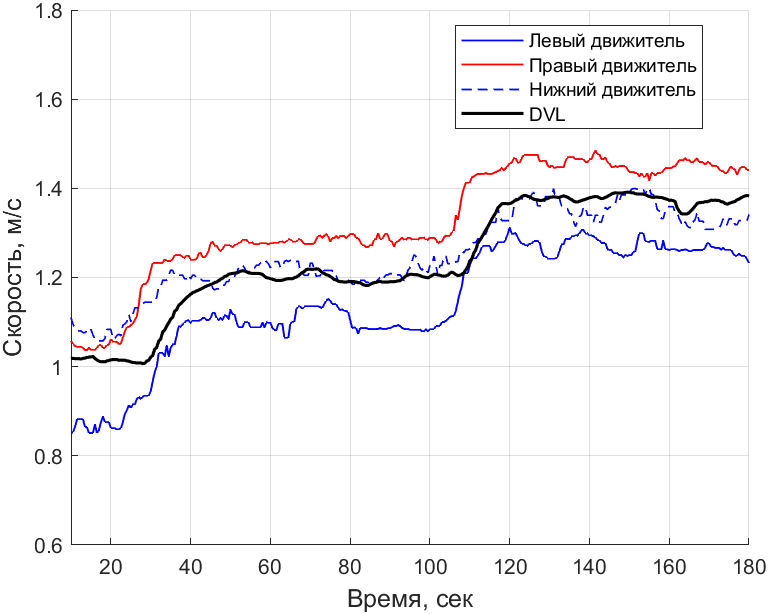
\includegraphics[width=0.8\linewidth]{velocity/MMT3000 - Скорость первый участок.png}
    \caption{Скорость продольного движения АНПА ``ММТ-3000'' от 0 до 185 секунд.}
    \label{fig:mmt3000_velocity_test}
\end{figure}

С помощью полученных коэффициентов была рассчитана скорость АНПА ``ММТ-3000'' на обратном пути движения в диапазоне времени от 240 до 410 секунд.
График скорости представлен на рисунке \ref{fig:mmt3000_velocity_check}.

\begin{figure}[ht]
    \centering
    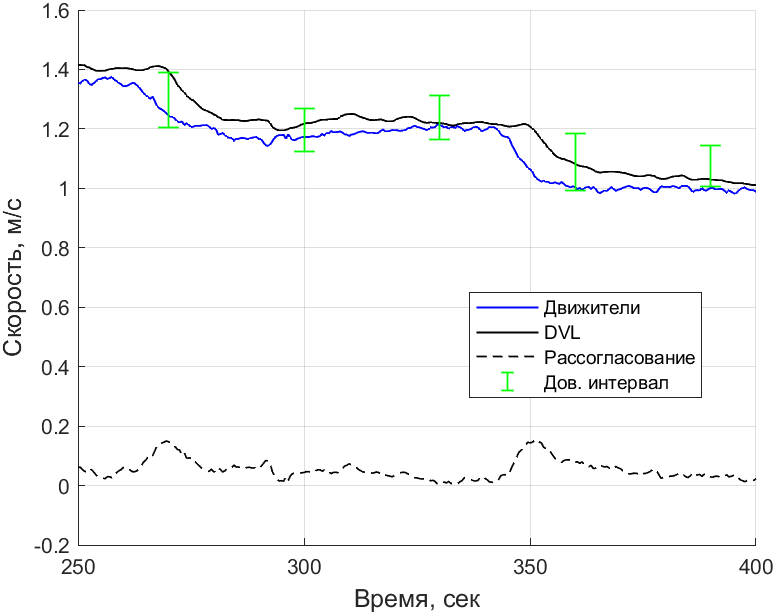
\includegraphics[width=0.8\linewidth]{velocity/ММТ3000 - тестирование b2.png}
    \caption{Cкорость продольного движения АНПА ``ММТ-3000'' на проверочном участке движения от 240 до 410 секунд.}
    \label{fig:mmt3000_velocity_check}
\end{figure}

\section{Выводы по главе 3}
Разработан метод оценки скорости набегающего потока в установившемся режиме движения АНПА по изменению параметров работы движителей маршевой группы.
Предложена методика уточнения параметров ГВ по результатам швартовных испытаний движителей и калибровочным запускам АНПА.

Предложенный метод позволяет оценить скорость движения АНПА относительно потока в случае отсутствия основного датчика скорости или выхода его из строя.

Была проведена верификация метода на обработке данных запусков АНПА ``ММТ-3000''.
После уточнения параметров ГВ на калибровочной части маршрута, расхождение оцениваемой скорости с эталонными показаниями доплеровского лага составило не более чем 0.18 м/с на переходных режимах и не более чем 0.1 м/с на установившихся режимах движения со среднеквадратичным отклонением $\sigma=0.17$ м/с.
